\section{Theoretical Foundation}

\subsection{Embeddings}
Word embeddings are a class of techniques in NLP where words or phrases from a vocabulary are mapped to vectors of real numbers. The core idea behind word embeddings is to capture the semantic meaning of words such that words with similar meanings have similar representations. This transformation allows machine learning algorithms to leverage the geometric properties of the embeddings, making it easier to analyze and process textual data. In the field of information retrieval, the first-stage retrieval often relies on text embeddings to efficiently recall a small set of candidate documents from a large-scale corpus using approximate nearest neighbor search techniques. Embedding-based retrieval is also a crucial component of RAG \cite{Wang.31Dec2023}.

The concept of representing words as vectors isn't entirely new. Its roots can be traced back to the 1950s and 1960s, with foundational work by linguists and cognitive scientists. The theoretical underpinning of word embeddings is the distributional hypothesis, which posits that words occurring in similar contexts tend to have similar meanings. This idea, often summarized as "You shall know a word by the company it keeps" \cite{J.R.Firth.1957}, forms the basis for various embedding techniques. By analyzing the contexts in which words appear, it is possible to infer their semantic properties.

The early attempts to quantify semantic similarity between words led to the development of thesauri and semantic networks, such as WordNet, which organized words based on their meanings and relationships. However, these approaches were largely symbolic and didn't capture the continuous nature of semantic relationships \cite{GeorgeA.Miller.1995}.

In the 1980s and 1990s, the introduction of Latent Semantic Analysis (LSA) marked a significant shift. At its core, LSA relies heavily on Singular Value Decomposition (SVD), a linear algebra technique that decomposes a matrix into three other matrices, allowing the extraction of latent semantic information. Specifically, LSA applies SVD to a term-document matrix, where each row corresponds to a term (word) and each column corresponds to a document. The entries of this matrix typically represent some measure of the frequency or importance of each term in each document. By performing SVD on this matrix, LSA identifies a set of orthogonal vectors (singular vectors) that capture the underlying patterns of co-occurrence between terms and documents. These vectors are ordered by the amount of variance they explain in the original data, enabling LSA to reduce the dimensionality of the term-document space while preserving the most significant patterns of word usage across documents. The output of LSA is a set of latent semantic vectors, where each term and document is represented as a vector in a lower-dimensional continuous space. This representation allows LSA to capture the semantic relationships between words and documents based on their distributional patterns across the corpus. One significant limitation of LSA is its scalability to large vocabularies. The term-document matrix grows with the number of unique terms in the corpus, resulting in a computational challenge when applying SVD. SVD is computationally expensive, especially for matrices with high dimensionality, making it impractical to scale LSA to very large datasets or vocabularies. LSA operates under the bag-of-words assumption, which means it disregards the order and context of words within documents. As a result, LSA may struggle to capture fine-grained contextual nuances and subtle differences in meaning that depend on word order or syntactic structure.

LSA pioneered the use of linear algebra techniques like SVD to uncover latent semantic structures in text data. Despite its success in capturing semantic relationships and reducing dimensionality, LSA has notable limitations. These include challenges with handling large vocabularies, capturing contextual nuances, potential information loss during dimensionality reduction, and lack of adaptability to changing linguistic contexts. These limitations paved the way for more advanced techniques like word embeddings (e.g., Word2Vec, GloVe) and contextualized embeddings (e.g., ELMo, BERT), which aim to address these shortcomings and provide richer representations of language in NLP tasks.

Another traditional approach for text-based learning is via the Term Frequency - Inverse Document Frequency (TF-IDF) method, which can represent the document as a long numeric vector of TF-IDF scores for each word. The TF-IDF is the product of two statistics, term frequency and inverse document frequency. There are various ways for determining the exact values of both statistics. However, TF-IDF does not attempt to directly extract the latent semantic information within the text.

The early 2000s saw further advancements with the introduction of neural network-based models. Some works on a neural probabilistic language model demonstrated that distributed representations of words could improve language modeling tasks \cite{YoshuaBengioRejeanDucharmePascalVincentChristianJauvin.2003}. This laid the groundwork for subsequent developments in word embeddings, leading to the creation of more sophisticated models like Word2Vec and GloVe.

Word2Vec is one of the most influential models for learning word embeddings. uses neural networks to generate word embeddings through two architectures: Continuous Bag of Words (CBOW) and Skip-gram \cite{Mikolov.16Jan2013}.

In the CBOW model, the objective is to predict a target word based on its surrounding context words. Formally, given a context window of size c, the probability of a target word \(w_{t}\) given the context words \\ \(w_{t-c}, \ldots, w_{t-1}, w_{t+1}, \ldots, w_{t+c}\) is modeled as:\\
\[P(w_t \mid w_{t-c}, \ldots, w_{t-1}, w_{t+1}, \ldots, w_{t+c})\] \\
The training involves maximizing the log probability of the target word given its context over the entire corpus.

The Skip-gram model, on the other hand, reverses this approach. It aims to predict the context words given a target word. For a given word \(w_{t}\), the model maximizes the probability of its surrounding words: \\
\[P(w_{t-c}, \ldots, w_{t-1}, w_{t+1}, \ldots, w_{t+c}) \mid w_t) \] \\
The Skip-gram model has been found to perform well, especially on smaller datasets and for capturing rare word representations. 

Both variants utilize negative sampling or hierarchical softmax to efficiently approximate the softmax function over a large vocabulary, making the training process computationally feasible.

GloVe (Global Vectors for Word Representation), combines the strengths of the count-based and prediction-based approaches. The core idea behind GloVe is to construct a global co-occurrence matrix from the corpus and then factorize this matrix to obtain word vectors \cite{Pennington.2014}.

The objective function in GloVe is designed to capture the ratio of word co-occurrence probabilities. Specifically, given a word \(w_i\) and a context word \(w_j\), the ratio of their co-occurrence probabilities with another word \(w_k\) should be similar to the ratio of their co-occurrence probabilities with each other. This relationship is captured by the following cost function: \\
\[
J = \sum_{i,j=1}^{V} f(X_{ij})(w_i^T w_j + b_i + b_j - \log X_{ij})^2
\]\\
Here, \(X_{ij}\) denotes the co-occurrence count of words \(w_i\) and \(w_j\), \(b_i\) and \(b_j\) are bias terms, and \(f(X_{ij})\) is a weighting function that limits the influence of frequent co-occurrences. By optimizing this objective function, GloVe learns embeddings that incorporate both local context (like Word2Vec) and global statistical information from the entire corpus.

FastText, developed by Facebook's AI Research (FAIR) lab, extends the Word2Vec model by representing words as bags of character n-grams \cite{Joulin.6Jul2016}. This approach allows FastText to capture subword information, making it particularly effective for morphologically rich languages and rare word representations. The model learns embeddings for character n-grams and represents words as the sum of these embeddings. The training process for FastText is similar to that of Word2Vec, but with the additional step of generating n-grams for each word. This modification enables FastText to generalize better to unseen words and handle out-of-vocabulary words more gracefully.

The above methods learn only a single, static representation for each word, and do not take into consideration the phenomenon of polysemy, where a word can change its meaning depending on the context. The state-of-the-art (SOTA) pre-trained language models built on top of the very effective Transformer-based attention model, which can learn contextual word embeddings. These embeddings are dynamic in terms of the surrounding block or context of the word, so that the same word can get different representations that are most effective in capturing the lexical and semantic information \cite{Xia.14Jun2022}. 

ELMo (Embeddings from Language Models) generates word embeddings based on the entire context of a sentence using bidirectional LSTM networks. ELMo is a deep contextualized word representation model designed to improve various NLP tasks by providing rich word embeddings. The key idea behind ELMo is to use representations from a bi-directional language model (biLM) that are learned from a large corpus. These representations are context-sensitive, meaning that they can capture different meanings of words depending on their usage in different sentences \cite{Peters.15Feb2018}.

BERT (Bidirectional Encoder Representations from Transformers) further improves contextual understanding by using the Transformer architecture \cite{Devlin.11Oct2018}. BERT alleviates the unidirectionality constraint (for example, a left-to-right architecture, where every token can only attend to previous tokens in the self-attention layers of the Transformer model) by using a “masked language model” (MLM) pre-training objective. The masked language model randomly masks some of the tokens from the input, and the objective is to predict the original vocabulary id of the masked word based only on its context. BERT’s model architecture is a multi-layer bidirectional Transformer \cite{Vaswani.12Jun2017} encoder with two model sizes: BERT(base)/  BERT(large) with 12/ 24 layers (transformer blocks), 768/ 1024 hidden size, 12/ 16 self-attention heads, 110M/ 340M total parameters, кespectively. 

BERT pre-trains a deep bidirectional model on large corpora, capturing intricate word relationships and achieving state-of-the-art performance on various NLP benchmarks. We will discuss the architecture of Transformers in more detail in the subsection of language models.

Recent research has introduced prominent embedding models such as AngIE, Voyage, BGE, etc, which are benefit from multi-task
instruct tuning. Hugging Face’s MTEB leaderboard evaluates embedding models across 8 tasks, covering 58 datasests. Additionally, C-MTEB focuses on Chinese capability, covering 6 tasks and 35 datasets. By the time of the experiments (March 2024), the small BGE model ('bge-small-en-v1.5') ranked high in the MTEB Leaderboard ranking \cite{Gao.18Dec2023}.

'bge-small-en-v1.5' uses BERT general architecture with 33.2 mln parameters, 512 context length (maximum tokens) and 384 embedding length (dimensions)\footnote{\url{https://ollama.com/znbang/bge:small-en-v1.5-f32/blobs/bf40c42ad7d8}}. The model uses a WordPiece tokenizer\footnote{\url{https://huggingface.co/BAAI/bge-small-en-v1.5/raw/main/tokenizer.json}}, which uses subword tokenization method, when single word might be broken down into smaller units called subtokens (similar to Byte Pair Encoding (BPE)).

BGE (BAAI General Embeddings) provides a family of welltrained models for English and Chinese general text embeddings. There are three optional model sizes: small (24M), base (102M), and large (326M). BGE model series have received more than 20 million downloads from HuggingFace since its release on August 2023, making it one of the most popular embedding models in the world. They have been integrated by the major RAG and text-embedding frameworks in the world, such as Langchain, LLamaIndex and Huggingface. The code-base also receives nearly 5,000 stars on GitHub \cite{Xiao.14Sep2023}.


\subsection{Transformers}
Recent advances in artificial intelligence, especially in natural language processing, have led to the development of powerful LLMs like ChatGPT. Over the past few decades, language model architectures have undergone significant evolution. Initially, n-gram models represented word sequences assuming that the probability of the next word depends solely on the preceding (n − 1) words. For example, in a bigram model, the probability of a word is only conditioned on the previous word. Later, Recurrent Neural Network (RNN)-based models like Long Short-Term Memory networks (LSTM) emerged as neural network solutions, which are capable of capturing long-term dependencies in sequential data \cite{.2023}.

A significant breakthrough came in 2017 with the introduction of the Transformer model \cite{Vaswani.12Jun2017}. Transformers are based on a processing concept called self-attention, an attention mechanism relating different positions of a single sequence in order to compute a representation of the sequence. Self-attention has been used successfully in a variety of tasks including reading comprehension, abstractive summarization, textual entailment and learning task-independent sentence representations. End-to-end memory networks are based on a recurrent attention mechanism instead of sequencealigned recurrence and have been shown to perform well on simple-language question answering and language modeling tasks. The Transformer is the first model relying entirely on self-attention to compute representations of its input and output without using sequence aligned RNNs or convolution \cite{AustinHuangSurajSubramanianJonathanSumKhalidAlmubarakandStellaBiderman..2022}.

The Transformer architecture is composed of an encoder-decoder structure, although many applications, such as BERT, use only the encoder, and others, like GPT, use only the decoder. The architecture is highly modular and consists of the following key components:
\begin{enumerate}
\item The Encoder processes the input sequence and generates a set of context-aware representations. It consists of multiple identical layers, each containing two main sub-layers Multi-Head Self-Attention Mechanism (allows the model to focus on different parts of the input sequence simultaneously by creating multiple attention heads. Each head computes a different attention distribution, and their outputs are concatenated and linearly transformed) and Position-Wise Feed-Forward Network(applies two linear transformations with an activation function in between to each position in the sequence independently, enhancing the model's ability to capture non-linear relationships. Each sub-layer is followed by layer normalization and residual connections to facilitate training and improve model stability.
\item The decoder generates the output sequence, often in an autoregressive manner, meaning it predicts the next word based on previously generated words and the encoder's context-aware representations. Similar to the encoder, the decoder consists of multiple identical layers, each containing three main sub-layers: Masked Multi-Head Self-Attention Mechanism (ensures that the prediction for a particular position depends only on the preceding positions, preserving the autoregressive property), Multi-Head Attention Mechanism (allows the decoder to attend to the encoder's output, integrating information from the input sequence) and Position-Wise Feed-Forward Network (operates similarly to its counterpart in the encoder). Like the encoder, each sub-layer in the decoder is followed by layer normalization and residual connections.
\item Since the Transformer does not inherently capture the order of words (due to its parallel processing nature), positional encoding is added to the input embeddings. This encoding provides information about the position of each word in the sequence, enabling the model to utilize the order of words. \cite{Vaswani.12Jun2017}
\end{enumerate}

The Transformer model employs a layered structure that includes multiple layers of self-attention mechanisms and fully connected neural networks in both its encoder and decoder components, as illustrated in the \autoref{fig:transformer}.

\begin{figure}[h!]
\centering
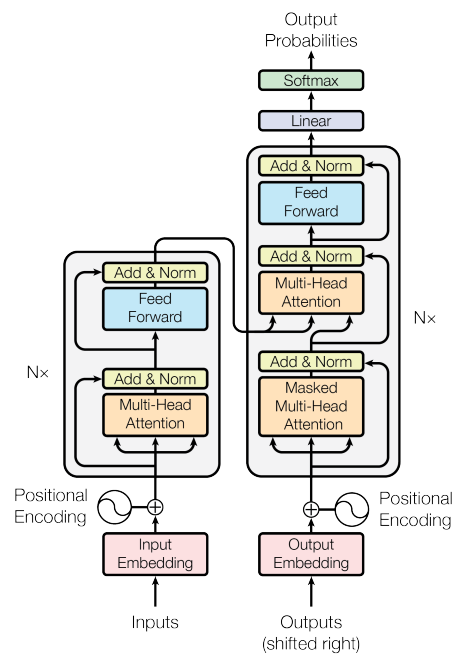
\includegraphics[width=0.5\textwidth]{Figures/transformer.png}
\caption{The Transformer architecture \cite{Vaswani.12Jun2017}.}
\label{fig:transformer}
\end{figure}

The original Transformer model architecture, as described in the paper \cite{Vaswani.12Jun2017}, comprises a stack of 6 identical layers for the encoder. Each encoder layer includes two sub-layers: the first is a multi-head self-attention mechanism, and the second is a position-wise fully connected feed-forward network. Every sub-layer in the encoder, along with the embedding layers, generates outputs with a dimensionality of 512.

Similarly, the decoder consists of a stack of 6 identical layers. Each layer in the decoder has the same two sub-layers as the encoder layers, with an additional third sub-layer. This third sub-layer performs multi-head attention over the output of the encoder stack. Multi-head attention is a module for attention mechanisms which runs through an attention mechanism several times in parallel. The independent attention outputs are then concatenated and linearly transformed into the expected dimension \cite{Vaswani.12Jun2017}.

Attention allows a network to give different weights to different inputs, with weighting coefficients that themselves depend on the input values, thereby capturing powerful inductive biases related to data. These models are known as transformers because they transform a set of vectors in some representation space into a corresponding set of vectors, having the same dimensionality, in some new space. The goal of the transformation is that the new space will have a richer internal representation that is better suited to solving downstream tasks. One major advantage of transformers is that transfer learning is very effective, so that a transformer model can be trained on a large body of data and then the trained model can be applied to many downstream tasks using some form of fine-tuning. Transformers can be trained in a self-supervised way using unlabelled data, and especially well suited to GPU allowing models having of the order of a trillion parameters to be trained in reasonable time. \cite{Bishop.2024}

The Generative Pre-trained Transformer (GPT) models, developed by OpenAI, are among the most prominent LLMs. GPT-2 demonstrated the power of unsupervised pre-training on diverse text corpora followed by fine-tuning on specific tasks. GPT-3, with 175 billion parameters, significantly advanced this approach, enabling highly coherent text generation and impressive zero-shot and few-shot learning capabilities \cite{Brown.28May2020}. In November 2022, OpenAI released the conversation model ChatGPT, based on the GPT models. And in March 2023 GPT-4 was
released, which extended the text input to multimodal signals (text, images, audios) \cite{Zhao.31Mar2023}.

The collection of LLaMA models were introduced by Meta AI in February, 2023, consisting of four sizes, ranging from 7B to 65B
parameters. \cite{Touvron.27Feb2023}. LLaMa results show that it is possible to achieve state-of-the-art performance by training
exclusively on publicly available data, without
resorting to proprietary datasets and moreover LLaMA-13B outperforms GPT-3 while being more than 10× smaller. In July, 2024 Meta introduced Llama 3.1 model with 128K tokens context length with three sizes 8B, 70B and a flagship model with 405B parameters. Llama 3.1 405B delivers comparable quality to leading language models such as GPT-4 on a plethora of tasks (general knowledge, steerability, math, tool use, and multilingual translation)\footnote{\url{https://ai.meta.com/research/publications/the-llama-3-herd-of-models/}}.  

The phi-3-mini model from Microsoft is a transformer decoder architecture, unlike the full Transformer architecture (which consists of both encoder and decoder components), the decoder-only architecture focuses on generating text by predicting the next word in a sequence based on the preceding context. The model's default context length is 4K tokens, which means the model can consider up to 4096 tokens of input context when making predictions \cite{Abdin.22Apr2024}. The phi-3-mini model is built using a block structure that is similar to the Llama-2 model \cite{Touvron.18Jul2023}. This ensures compatibility and ease of adaptation for tools and techniques developed for Llama-2. The model uses the same tokenizer with vocabulary size of 320641. The tokenizer is responsible for converting text into tokens that the model can process. The vocabulary size indicates the number of unique tokens the model can recognize and generate. This large vocabulary size helps the model handle a diverse range of words and phrases.

The model uses 3072 hidden dimension (refers to the size of the hidden layers in the model, indicates the number of units in each hidden layer, which affects the model's capacity to learn and represent complex patterns in the data), 32 heads (determines how many different attention distributions are computed. Using 32 heads means that the model can focus on 32 different aspects of the input context simultaneously, enhancing its ability to capture nuanced relationships between tokens) and 32 layers stacked on top of each other (each layer contains its own set of parameters and contributes to the model's depth, enabling it to learn hierarchical representations of the input data). 

The model is trained using bfloat16 (Brain Floating Point, a 16-bit floating-point format provides a good balance between computational efficiency and numerical precision) for a total of 3.3T tokens (a larger training corpus provides the model with more diverse language patterns and knowledge, improving its ability to generate high-quality text). Developers utilized high quality training data to improve the performance of small language model. Such method allowed to reach the level of highly capable models such as GPT-3.5 or Mixtral with only 3.8B total parameters (while Mixtral has 45B total parameters). Phi-3 model's training data consists of heavily filtered publicly available web data from various open internet sources, as
well as synthetic LLM-generated data. Thanks to its small size, phi3-mini can be quantized to 4-bits so that it only occupies ≈ 1.8GB of memory. \cite{Abdin.22Apr2024}

In terms of LLM capabilities, while phi-3-mini model achieves similar level of language understanding and reasoning ability as much larger models, it is still fundamentally limited by its size for certain tasks. The model simply does not have the capacity to store too much “factual knowledge”. Moreover, developers have identified certain limitations, particularly with questions necessitating high-level reasoning abilities. Additionally, the model has been observed to occasionally generate ungrounded outputs, making it potentially unreliable in sensitive areas, such as finance. Such weakness can be resolved by augmentation with a search engine. \cite{Abdin.22Apr2024}


\subsection{Vector Databases}
A vector database is a database designed to store data as high-dimensional vectors, which mathematically represent features or attributes. Each vector comprises numerous dimensions, ranging from tens to thousands, depending on the data's complexity and detail. These vectors are typically created by applying an embedding function to the raw text \cite{Han.18Oct2023}. 

Vector databases function by building an index for all vectors contained within the database. This index is organized according to the vectors' attributes and their similarities. When a query is made to retrieve a vector, the database searches the index to find the most similar vectors and returns them as results. This approach allows for quick and efficient vector retrieval, even in large and complex databases. 

There are two primary approaches for searching in vector databases: Nearest Neighbor Search (NNS) and its variant, Approximate Nearest Neighbor Search (ANNS).

NNS is an optimization problem focused on identifying the point in a given dataset that is closest or most similar to a specified query point. Closeness is typically evaluated using a dissimilarity function, where larger function values indicate less similarity. For example, NNS can be utilized to locate documents similar to a specified document based on topic and sentiment. NNS algorithms usually employ exact or deterministic methods. Some common techniques include: "k-d tree" method partitions the space into regions by splitting along one dimension at a time; "Ball tree" approach encloses groups of points within hyperspheres. These methods visit only the regions that may contain the nearest neighbor, based on certain distance bounds or criteria \cite{Han.18Oct2023}.

ANNS, in contrast, allows for some approximation or error in the search results, trading off accuracy for increased speed and space efficiency. This approach is particularly advantageous for handling large-scale and high-dimensional data. ANNS methods use more probabilistic or heuristic strategies, such as: "Locality-sensitive hashing (LSH)" maps similar points to the same or nearby buckets with high probability; "Best bin first" visits regions in order of their distance to the query point and stops after examining a fixed number of regions or points; "Hierarchical navigable small world (HNSW)" follows edges that lead to closer points in a graph with different levels of coarseness \cite{Han.18Oct2023}.

The primary difference between NNS and ANNS algorithms lies in their design principles. NNS algorithms organize the data into exact structures and traverse these structures to find the nearest neighbor deterministically. ANNS algorithms use approximate structures and probabilistic methods to quickly find a close, but not necessarily the exact, nearest neighbor.
Any data structure or algorithm that supports NNS can generally be adapted for ANNS, offering flexibility for various search requirements. This adaptability ensures that vector databases can efficiently handle diverse and complex queries, making them suitable for a wide range of applications in fields like image retrieval, document clustering, and recommendation systems \cite{Han.18Oct2023}.

Hierarchical Navigable Small World (HNSW) is an advanced method for approximate nearest neighbor search in high-dimensional vector collections. It employs a graph structure where nodes represent vectors and edges denote similarity or distance. The algorithm uses a greedy search strategy, starting from a random point and moving to its nearest neighbor until no closer point is found. HNSW follows the following formula for finding the nearest neighbor of a point p in the graph using a random walk:
\[
\arg\min_{q \in N(p)} d(p, q)
\]
where \(N_p\) is the set of neighbors of \(p\) in the graph, and
\(d\) is a distance function, such as Euclidean distance or cosine
distance.

Adding edges to the graph follows a heuristic where points closer to a node than its current neighbors are connected:
\[
\forall q \in \mathcal{N}(p), \forall r \in \mathcal{N}(q), \text{ if } d(p, r) < d(p, q), \text{ then add edge}(p, r)
\]
where \(N_p\) and \(N_q\) are the sets of neighbors of \(p\) and
\(q\) in the graph, respectively, and \(d\) is a distance function.

HNSW organizes vectors into layers with different densities and distances, controlled by a parameter \(M\). Higher layers contain fewer nodes with longer edges, while lower layers have more nodes with shorter edges. Search begins at the highest layer, progressively refining candidates at each layer until the nearest neighbor is found. The formula for assigning a point \(p\) to a layer \(l\) using a random probability is:
\[
\Pr[p \in l] = \begin{cases}
1 & \text{if } l = 0, \\
\frac{1}{M} & \text{if } l > 0.
\end{cases}
\]
where \(M\) is the parameter that controls the maximum number of neighbors for each point in each layer. The algorithm assigns \(p\) to layer \(l\) with probability \(\Pr[p \in l]\), and stops when it fails to assign p to any higher layer. The formula for searching for the nearest neighbor of a query point \(q\) in the hierarchical graph is:
\[
\min_{p \in C(q)} d(q, p)
\]
where \(C_q\) is the set of candidate points obtained by
traversing each layer of the graph from top to bottom and
retrieving all the points that are closer than the current best
distance.

Key advantages of HNSW include its ability to handle various distance metrics, adapt to dynamic datasets, and achieve high accuracy with low memory usage compared to tree-based or hash-based methods. However, its performance depends on factors like vector dimensionality, layer count, neighbor count, and query hop count, impacting trade-offs between accuracy and efficiency \cite{Han.18Oct2023}.

Several open-source vector databases are available under Apache 2.0 or MIT licenses, including Chroma, Faiss, Marqo, Vespa, Qdrant, LanceDB, and Milvus. Additionally, traditional databases such as OpenSearch, ClickHouse (a column-oriented DBMS), PostgreSQL, and Cassandra now offer support for vector search. Although we did not conduct an in-depth analysis of these databases, we selected ChromaDB due to its simplicity and ease of use.

ChromaDB's straightforward integration makes it a good choice for our purpose, allowing us to focus on our core research objectives without being encumbered by complex database configurations. ChromaDB utilizes SQLite to store vectors in its in-memory version. SQLite, a file-based relational database, inherently lacks support for vector data. When a document is added to a collection, ChromaDB employs an embedding function to generate vectors for the document. For each collection, an index is constructed using the HNSW (Hierarchical Navigable Small World) approximate nearest neighbor search algorithm. When a text string is queried within a collection, ChromaDB generates vectors for the string using the same embedding function. It then searches the index for the k nearest neighbors, with k specified in the query. The index maintains UUIDs for the documents, which are used to retrieve the corresponding text strings.


\subsection{Retriever-Augmented Generation}
LLMs have demonstrated impressive performance, yet they still encounter notable challenges, particularly with tasks that require specialized knowledge or up-to-date information. A common issue is that they may produce "hallucinations"—inaccurate or fabricated information—when faced with queries that extend beyond their training data or require current facts. To address these limitations, RAG has been developed to improve LLMs. RAG enhances the capabilities of LLMs by retrieving relevant sections from an external knowledge base based on semantic similarity. This approach helps mitigate the generation of factually incorrect content by incorporating accurate external information. The adoption of RAG in LLMs has become widespread, positioning it as a crucial technology for advancing chatbots and making LLMs more effective and reliable for real-world applications \cite{Gao.18Dec2023}. 

The field of RAG has evolved swiftly in recent years, exhibiting several distinct phases of development in the context of large models. Initially, RAG emerged alongside the rise of the Transformer architecture, focusing on improving language models by integrating additional knowledge through Pre-Training Models (PTM). This early phase was dedicated to advancing pre-training methods and laying a solid foundation. The introduction of ChatGPT marked a significant turning point, showcasing advanced in-context learning (ICL) capabilities. This development prompted a shift in RAG research toward enhancing the provision of relevant information for LLMs, enabling them to handle more complex and knowledge-intensive tasks during the inference phase. As a result, RAG research experienced rapid advancements. Over time, improvements in RAG extended beyond just the inference stage and began to integrate with techniques for fine-tuning LLMs, reflecting a broader evolution in the field \cite{Gao.18Dec2023}.

A typical application of RAG is illustrated in the \autoref{fig:RAG}:
\begin{figure}[h!]
\centering
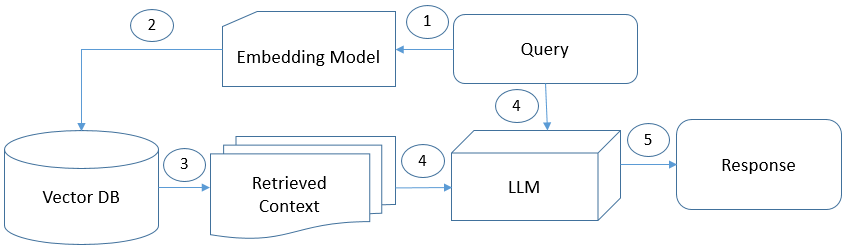
\includegraphics[width=1\textwidth]{Figures/RAG.png}
\caption{A typical RAG architecture}
\label{fig:RAG}
\end{figure}


Here, the user initiates the process by submitting a query (question or request). The query is then passed through an embedding model, which transforms the text data into a numerical representation. This allows the model to identify similar text passages within the document collection. The embedding model interacts with a vector database to retrieve relevant documents or passages. The vector database efficiently stores and retrieves information based on the numerical representations generated by the embedding model. The retrieved documents or passages that are most relevant to the query are then incorporated into the workflow. The retrieved context is presented, along with the original query, to a LLM. LLMs are trained on massive amounts of text data and are adept at understanding and responding to natural language. In the RAG workflow, the LLM leverages the retrieved context to generate a comprehensive and informative response to the user’s query. Finally, the LLM’s response is provided to the user.

Mathematically, the task of the RAG system can be formulated as follows.  Given input \(X\) and an accessible corpus containing a large amount of knowledge documents \(C = \{d_1, \ldots, d_N\}\), the system is expected to generate the output \(Y\). The entire framework is divided into a retriever \(R\)
and a generator \(G\). The retriever \(R\) aims to retrieve
the top-K documents \(D = \{d_{r1}, \ldots, d_{rk}\}\) that are
relevant to the input \(X\) from the corpus \(C\). Based on the input \(X\) and the retrieved results \(D\), the generator \(G\) is responsible for generating the output \(Y\). This framework can be formulated as:

\[P(Y|X) = P(D|X)P(Y, D|X)\]

It shows that the retriever and generator are seamlessly coupled, exhibiting low risk tolerance. Any unsuccessful retrieval can result in an unsatisfactory response, regardless of the impressive abilities of the generator \cite{Yan.29Jan2024}.

The RAG research paradigm is continuously evolving, and it may categorized into three stages: Naive RAG, Advanced RAG, and Modular RAG. Despite RAG method are cost-effective and surpass the performance of the native LLM, they also exhibit several limitations. The development of Advanced RAG and Modular RAG is a response to these specific shortcomings in Naive RAG. \cite{Gao.18Dec2023}

The Naive RAG research paradigm represents the earliest methodology, which gained prominence shortly after the widespread adoption of ChatGPT. The Naive RAG follows a traditional process that includes indexing, retrieval, and generation, which is also characterized as a “Retrieve-Read” framework. 

Indexing starts with the cleaning and extraction of raw data in diverse formats, which is then converted into a uniform plain text format. To accommodate the context limitations of language models, text is segmented into smaller, digestible chunks. Chunks are then encoded into vector representations using an embedding model and stored in vector database. This step is crucial for enabling efficient similarity searches in the subsequent retrieval phase. 

Upon receipt of a user query, the RAG system employs the same encoding model utilized during the indexing phase to transform the query into a vector representation. It then computes the similarity scores between the query vector and the vector of chunks within the indexed corpus. The system prioritizes and retrieves the top K chunks that demonstrate the greatest similarity to the query. These chunks are subsequently used as the expanded context in prompt. 

The posed query and selected documents are synthesized into a coherent prompt to which a large language model is tasked with formulating a response. The model’s approach to answering may vary depending on task-specific criteria, allowing it to either draw upon its inherent parametric knowledge or restrict its responses to the information contained within the provided documents \cite{Gao.18Dec2023}.

Naive RAG approaches face several significant challenges. During the retrieval phase, issues with precision and recall often arise, leading to the selection of irrelevant or mismatched chunks and missing important information. In the response generation phase, the model might produce hallucinations—content that is not supported by the retrieved context. This stage can also suffer from problems such as irrelevance, toxicity, or bias in the generated responses, which undermines the overall quality and reliability. Combining the retrieved information with the specific task at hand can be difficult, occasionally resulting in fragmented or incoherent responses. Additionally, there may be redundancy when similar information is retrieved from multiple sources, causing repetitive outputs. Assessing the significance and relevance of different passages, and maintaining stylistic and tonal consistency, further complicates the process. Moreover, a single retrieval based on the initial query might not provide sufficient context. There is also a risk that generation models may excessively rely on the retrieved information, producing outputs that merely restate the retrieved content without offering new insights or synthesis\cite{Gao.18Dec2023}.

Advanced RAG introduces specific improvements to overcome the limitations of Naive RAG. Focusing on enhancing retrieval quality, it employs pre-retrieval and post-retrieval strategies. The typical advanced RAG architecture is shown in \autoref{fig:advanced_arch}.\\ 
\begin{figure}[h!]
\centering
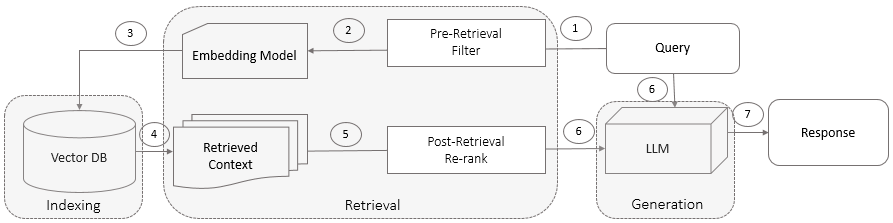
\includegraphics[width=1\textwidth]{Figures/advanced_arch.png}
\caption{An advanced RAG architecture}
\label{fig:advanced_arch}
\end{figure}

In the pre-retrieval stage, the main objectives are to optimize both the indexing structure and the original query. Improving the indexing involves enhancing the quality of the content that is indexed, often through techniques such as metadata filtering. On the other hand, optimizing the query aims to clarify and refine the user's question to better align it with the retrieval task. Once relevant information has been retrieved, it is crucial to integrate it effectively with the original query. The post-retrieval process focuses on methods such as re-ranking the retrieved content. Re-ranking involves adjusting the position of retrieved information to ensure the most pertinent content is prioritized. This approach is utilized in frameworks like LlamaIndex and LangChain. To avoid information overload, where excessive or irrelevant content can obscure key details, post-retrieval efforts are directed toward selecting only the most critical information. This includes highlighting essential sections and condensing the context to ensure that the most relevant details are processed effectively \cite{Gao.18Dec2023}.

Evaluating RAG systems involves examining specific components and the overall complexity of the system, beyond just its primary functions of Retrieval and Generation. The retrieval component is essential for obtaining relevant information that guides the generation process. Traditional retrieval evaluation metrics like Recall and Precision are insufficient for capturing the nuances of RAG systems, thus necessitating the creation of more nuanced and task-specific metrics.

The challenge with the Generation component is to assess the faithfulness and accuracy of the generated content relative to the input data. This means evaluating not only the factual correctness of responses but also their relevance to the original query and the coherence of the generated text. Evaluating the entire RAG system introduces additional complexities. It requires assessing how well the system leverages retrieved information to enhance response quality, which involves measuring the added value of the retrieval component to the generative process. Challenges also arise in developing metrics that encompass generative evaluation criteria for various downstream tasks, human preferences, and practical considerations within the RAG system. Different targets necessitate different metrics suited to the specific datasets. For retrieval evaluation, the focus is on metrics that accurately capture the relevance, accuracy, diversity, and robustness of the information retrieved. These metrics must reflect the system’s precision in fetching pertinent information and its resilience in navigating the dynamic, vast, and sometimes misleading landscape of available data \cite{Yu.13May2024}. 

Non-Rank Based Metrics often assess binary outcomes—whether an item is relevant or not—without considering its position in a ranked list. Accuracy measures the proportion of true results among the total cases examined. Precision is the fraction of relevant instances among the retrieved instances. Recall at k (Recall@k) is the fraction of relevant instances retrieved out of the total relevant cases, considering only the top k results.

Rank-Based Metrics evaluate the order in which relevant items are presented, giving higher importance to the positioning of relevant items. Mean Reciprocal Rank (MRR) is the average of the reciprocal ranks of the first correct answer for a set of queries. Mean Average Precision (MAP) is the mean of the average precision scores for each query.

In the realm of generation, evaluation extends beyond the accuracy of generated responses to include text quality in terms of coherence, relevance, fluency, and alignment with human judgment. This requires metrics that assess the nuanced aspects of language production, such as factual correctness, readability, and user satisfaction with the generated content. Traditional metrics like BLEU, ROUGE, and F1 Score remain important, emphasizing precision and recall in determining response quality. However, new metrics such as Misleading Rate, Mistake Reappearance Rate, and Error Detection Rate highlight the evolving understanding of RAG systems’ unique challenges. Human evaluation continues to be a significant standard for comparing the performance of generation models with one another and with the ground truth \cite{Yu.13May2024}.